% Options for packages loaded elsewhere
\PassOptionsToPackage{unicode}{hyperref}
\PassOptionsToPackage{hyphens}{url}
\PassOptionsToPackage{dvipsnames,svgnames,x11names}{xcolor}
%
\documentclass[
  letterpaper,
  DIV=11,
  numbers=noendperiod]{scrreprt}

\usepackage{amsmath,amssymb}
\usepackage{iftex}
\ifPDFTeX
  \usepackage[T1]{fontenc}
  \usepackage[utf8]{inputenc}
  \usepackage{textcomp} % provide euro and other symbols
\else % if luatex or xetex
  \usepackage{unicode-math}
  \defaultfontfeatures{Scale=MatchLowercase}
  \defaultfontfeatures[\rmfamily]{Ligatures=TeX,Scale=1}
\fi
\usepackage{lmodern}
\ifPDFTeX\else  
    % xetex/luatex font selection
\fi
% Use upquote if available, for straight quotes in verbatim environments
\IfFileExists{upquote.sty}{\usepackage{upquote}}{}
\IfFileExists{microtype.sty}{% use microtype if available
  \usepackage[]{microtype}
  \UseMicrotypeSet[protrusion]{basicmath} % disable protrusion for tt fonts
}{}
\makeatletter
\@ifundefined{KOMAClassName}{% if non-KOMA class
  \IfFileExists{parskip.sty}{%
    \usepackage{parskip}
  }{% else
    \setlength{\parindent}{0pt}
    \setlength{\parskip}{6pt plus 2pt minus 1pt}}
}{% if KOMA class
  \KOMAoptions{parskip=half}}
\makeatother
\usepackage{xcolor}
\usepackage[heightrounded]{geometry}
\setlength{\emergencystretch}{3em} % prevent overfull lines
\setcounter{secnumdepth}{-\maxdimen} % remove section numbering
% Make \paragraph and \subparagraph free-standing
\ifx\paragraph\undefined\else
  \let\oldparagraph\paragraph
  \renewcommand{\paragraph}[1]{\oldparagraph{#1}\mbox{}}
\fi
\ifx\subparagraph\undefined\else
  \let\oldsubparagraph\subparagraph
  \renewcommand{\subparagraph}[1]{\oldsubparagraph{#1}\mbox{}}
\fi

\usepackage{color}
\usepackage{fancyvrb}
\newcommand{\VerbBar}{|}
\newcommand{\VERB}{\Verb[commandchars=\\\{\}]}
\DefineVerbatimEnvironment{Highlighting}{Verbatim}{commandchars=\\\{\}}
% Add ',fontsize=\small' for more characters per line
\newenvironment{Shaded}{}{}
\newcommand{\AlertTok}[1]{\textcolor[rgb]{1.00,0.33,0.33}{\textbf{#1}}}
\newcommand{\AnnotationTok}[1]{\textcolor[rgb]{0.42,0.45,0.49}{#1}}
\newcommand{\AttributeTok}[1]{\textcolor[rgb]{0.84,0.23,0.29}{#1}}
\newcommand{\BaseNTok}[1]{\textcolor[rgb]{0.00,0.36,0.77}{#1}}
\newcommand{\BuiltInTok}[1]{\textcolor[rgb]{0.84,0.23,0.29}{#1}}
\newcommand{\CharTok}[1]{\textcolor[rgb]{0.01,0.18,0.38}{#1}}
\newcommand{\CommentTok}[1]{\textcolor[rgb]{0.42,0.45,0.49}{#1}}
\newcommand{\CommentVarTok}[1]{\textcolor[rgb]{0.42,0.45,0.49}{#1}}
\newcommand{\ConstantTok}[1]{\textcolor[rgb]{0.00,0.36,0.77}{#1}}
\newcommand{\ControlFlowTok}[1]{\textcolor[rgb]{0.84,0.23,0.29}{#1}}
\newcommand{\DataTypeTok}[1]{\textcolor[rgb]{0.84,0.23,0.29}{#1}}
\newcommand{\DecValTok}[1]{\textcolor[rgb]{0.00,0.36,0.77}{#1}}
\newcommand{\DocumentationTok}[1]{\textcolor[rgb]{0.42,0.45,0.49}{#1}}
\newcommand{\ErrorTok}[1]{\textcolor[rgb]{1.00,0.33,0.33}{\underline{#1}}}
\newcommand{\ExtensionTok}[1]{\textcolor[rgb]{0.84,0.23,0.29}{\textbf{#1}}}
\newcommand{\FloatTok}[1]{\textcolor[rgb]{0.00,0.36,0.77}{#1}}
\newcommand{\FunctionTok}[1]{\textcolor[rgb]{0.44,0.26,0.76}{#1}}
\newcommand{\ImportTok}[1]{\textcolor[rgb]{0.01,0.18,0.38}{#1}}
\newcommand{\InformationTok}[1]{\textcolor[rgb]{0.42,0.45,0.49}{#1}}
\newcommand{\KeywordTok}[1]{\textcolor[rgb]{0.84,0.23,0.29}{#1}}
\newcommand{\NormalTok}[1]{\textcolor[rgb]{0.14,0.16,0.18}{#1}}
\newcommand{\OperatorTok}[1]{\textcolor[rgb]{0.14,0.16,0.18}{#1}}
\newcommand{\OtherTok}[1]{\textcolor[rgb]{0.44,0.26,0.76}{#1}}
\newcommand{\PreprocessorTok}[1]{\textcolor[rgb]{0.84,0.23,0.29}{#1}}
\newcommand{\RegionMarkerTok}[1]{\textcolor[rgb]{0.42,0.45,0.49}{#1}}
\newcommand{\SpecialCharTok}[1]{\textcolor[rgb]{0.00,0.36,0.77}{#1}}
\newcommand{\SpecialStringTok}[1]{\textcolor[rgb]{0.01,0.18,0.38}{#1}}
\newcommand{\StringTok}[1]{\textcolor[rgb]{0.01,0.18,0.38}{#1}}
\newcommand{\VariableTok}[1]{\textcolor[rgb]{0.89,0.38,0.04}{#1}}
\newcommand{\VerbatimStringTok}[1]{\textcolor[rgb]{0.01,0.18,0.38}{#1}}
\newcommand{\WarningTok}[1]{\textcolor[rgb]{1.00,0.33,0.33}{#1}}

\providecommand{\tightlist}{%
  \setlength{\itemsep}{0pt}\setlength{\parskip}{0pt}}\usepackage{longtable,booktabs,array}
\usepackage{calc} % for calculating minipage widths
% Correct order of tables after \paragraph or \subparagraph
\usepackage{etoolbox}
\makeatletter
\patchcmd\longtable{\par}{\if@noskipsec\mbox{}\fi\par}{}{}
\makeatother
% Allow footnotes in longtable head/foot
\IfFileExists{footnotehyper.sty}{\usepackage{footnotehyper}}{\usepackage{footnote}}
\makesavenoteenv{longtable}
\usepackage{graphicx}
\makeatletter
\def\maxwidth{\ifdim\Gin@nat@width>\linewidth\linewidth\else\Gin@nat@width\fi}
\def\maxheight{\ifdim\Gin@nat@height>\textheight\textheight\else\Gin@nat@height\fi}
\makeatother
% Scale images if necessary, so that they will not overflow the page
% margins by default, and it is still possible to overwrite the defaults
% using explicit options in \includegraphics[width, height, ...]{}
\setkeys{Gin}{width=\maxwidth,height=\maxheight,keepaspectratio}
% Set default figure placement to htbp
\makeatletter
\def\fps@figure{htbp}
\makeatother

\usepackage{fvextra}
\DefineVerbatimEnvironment{Highlighting}{Verbatim}{breaklines,commandchars=\\\{\}}
\KOMAoption{captions}{tableheading}
\makeatletter
\@ifpackageloaded{tcolorbox}{}{\usepackage[skins,breakable]{tcolorbox}}
\@ifpackageloaded{fontawesome5}{}{\usepackage{fontawesome5}}
\definecolor{quarto-callout-color}{HTML}{909090}
\definecolor{quarto-callout-note-color}{HTML}{0758E5}
\definecolor{quarto-callout-important-color}{HTML}{CC1914}
\definecolor{quarto-callout-warning-color}{HTML}{EB9113}
\definecolor{quarto-callout-tip-color}{HTML}{00A047}
\definecolor{quarto-callout-caution-color}{HTML}{FC5300}
\definecolor{quarto-callout-color-frame}{HTML}{acacac}
\definecolor{quarto-callout-note-color-frame}{HTML}{4582ec}
\definecolor{quarto-callout-important-color-frame}{HTML}{d9534f}
\definecolor{quarto-callout-warning-color-frame}{HTML}{f0ad4e}
\definecolor{quarto-callout-tip-color-frame}{HTML}{02b875}
\definecolor{quarto-callout-caution-color-frame}{HTML}{fd7e14}
\makeatother
\makeatletter
\@ifpackageloaded{caption}{}{\usepackage{caption}}
\AtBeginDocument{%
\ifdefined\contentsname
  \renewcommand*\contentsname{Table of contents}
\else
  \newcommand\contentsname{Table of contents}
\fi
\ifdefined\listfigurename
  \renewcommand*\listfigurename{List of Figures}
\else
  \newcommand\listfigurename{List of Figures}
\fi
\ifdefined\listtablename
  \renewcommand*\listtablename{List of Tables}
\else
  \newcommand\listtablename{List of Tables}
\fi
\ifdefined\figurename
  \renewcommand*\figurename{Figure}
\else
  \newcommand\figurename{Figure}
\fi
\ifdefined\tablename
  \renewcommand*\tablename{Table}
\else
  \newcommand\tablename{Table}
\fi
}
\@ifpackageloaded{float}{}{\usepackage{float}}
\floatstyle{ruled}
\@ifundefined{c@chapter}{\newfloat{codelisting}{h}{lop}}{\newfloat{codelisting}{h}{lop}[chapter]}
\floatname{codelisting}{Listing}
\newcommand*\listoflistings{\listof{codelisting}{List of Listings}}
\makeatother
\makeatletter
\makeatother
\makeatletter
\@ifpackageloaded{caption}{}{\usepackage{caption}}
\@ifpackageloaded{subcaption}{}{\usepackage{subcaption}}
\makeatother
\makeatletter
\@ifpackageloaded{tcolorbox}{}{\usepackage[skins,breakable]{tcolorbox}}
\makeatother
\makeatletter
\@ifundefined{shadecolor}{\definecolor{shadecolor}{HTML}{31BAE9}}{}
\makeatother
\makeatletter
\makeatother
\makeatletter
\ifdefined\Shaded\renewenvironment{Shaded}{\begin{tcolorbox}[boxrule=0pt, breakable, sharp corners, enhanced, borderline west={3pt}{0pt}{shadecolor}, interior hidden, frame hidden]}{\end{tcolorbox}}\fi
\makeatother
\ifLuaTeX
  \usepackage{selnolig}  % disable illegal ligatures
\fi
\usepackage{bookmark}

\IfFileExists{xurl.sty}{\usepackage{xurl}}{} % add URL line breaks if available
\urlstyle{same} % disable monospaced font for URLs
\hypersetup{
  colorlinks=true,
  linkcolor={blue},
  filecolor={Maroon},
  citecolor={Blue},
  urlcolor={Blue},
  pdfcreator={LaTeX via pandoc}}

\author{}
\date{}

\begin{document}

\RecustomVerbatimEnvironment{verbatim}{Verbatim}{
  showspaces = false,
  showtabs = false,
  breaksymbolleft={},
  breaklines
}

\renewcommand*\contentsname{Table of contents}
{
\hypersetup{linkcolor=}
\setcounter{tocdepth}{2}
\tableofcontents
}
\chapter{Using an HPC}\label{using-an-hpc}

Now, that we are familiar with using the cli, let's upload our
sequencing data to an HPC an run some software to check the quality of
our reads.

\section{\texorpdfstring{\texttt{ssh}: Connecting to a
sever}{ssh: Connecting to a sever}}\label{ssh-connecting-to-a-sever}

\textbf{SSH} (Secure Shell) is a network protocol that enables secure
remote connections between two systems. The basic command to login looks
like this:

\begin{Shaded}
\begin{Highlighting}[]
\CommentTok{\#connect to a server}
\FunctionTok{ssh} \AttributeTok{{-}X}\NormalTok{ username@server}
\end{Highlighting}
\end{Shaded}

Options:

\begin{itemize}
\tightlist
\item
  \texttt{-X} option enables untrusted X11 forwarding in SSH. Untrusted
  means = your local client sends a command to the remote machine and
  receives the graphical output. We use it since it enables users to run
  graphical applications on a remote server
\end{itemize}

If you have access to and want to connect to crunchomics you would
connect like this:

\begin{Shaded}
\begin{Highlighting}[]
\FunctionTok{ssh} \AttributeTok{{-}X}\NormalTok{ uvanetid1@omics{-}h0.science.uva.nl}
\end{Highlighting}
\end{Shaded}

\begin{tcolorbox}[enhanced jigsaw, coltitle=black, leftrule=.75mm, colback=white, toptitle=1mm, breakable, toprule=.15mm, colbacktitle=quarto-callout-important-color!10!white, bottomtitle=1mm, arc=.35mm, opacitybacktitle=0.6, bottomrule=.15mm, titlerule=0mm, title=\textcolor{quarto-callout-important-color}{\faExclamation}\hspace{0.5em}{Important}, rightrule=.15mm, left=2mm, colframe=quarto-callout-important-color-frame, opacityback=0]

If you want to log into Crunchomics from outside of UvA you need to be
connected to the VPN. If you have not set that up and/or have trouble
doing so, contact ICT.

\end{tcolorbox}

\section{Crunchomics: Preparing your
account}\label{crunchomics-preparing-your-account}

If you have not used Crunchomics before, then you want to run a small
Bash script that:

\begin{itemize}
\tightlist
\item
  Allows you to use system-wide installed software, by adding
  \texttt{/zfs/omics/software/bin} to your path. This basically means
  that bash knows that there is an extra folder in which to look for any
  software that is already installed
\item
  Sets up a python3 environment and some usefull python packages
\item
  Have a link for your 500 GB personal directory in your home directory
\end{itemize}

To set this up, run the following in the cli:

\begin{Shaded}
\begin{Highlighting}[]
\ExtensionTok{/zfs/omics/software/script/omics\_install\_script}
\end{Highlighting}
\end{Shaded}

\section{\texorpdfstring{\texttt{scp}: Transferring data from/to a
server}{scp: Transferring data from/to a server}}\label{scp-transferring-data-fromto-a-server}

\texttt{scp} stands for Secure Copy Protocol and allows us to securely
copy files and directories between remote hosts. When transferring data
the transfer is prepared from the terminal of your local computer and
not from the HPCs login node.

The basic syntax is:

\texttt{scp\ {[}options{]}\ SOURCE\ DESTINATION}

To start analysing our data, we want to move our fastq.gz files from our
local folder, the source, to a folder on Cruncomics, the destination.
Let's start by:

\begin{itemize}
\tightlist
\item
  Moving from our home directory into our personal directory. We move
  there since we have more space in the personal directory. Notice, for
  bash to find the personal directory, we need to have run the
  \texttt{omics\_install\_script} script above first
\item
  Make a project folder with a descriptive file name
\end{itemize}

\begin{Shaded}
\begin{Highlighting}[]
\BuiltInTok{cd}\NormalTok{ personal/}
\FunctionTok{mkdir}\NormalTok{ projectX}
\BuiltInTok{cd}\NormalTok{ projectX}
\end{Highlighting}
\end{Shaded}

Into our project directory, we the want to move the data we have before
downloaded with our sequencing data. We do this by moving the
\texttt{data} folder we generated before from our local computer to the
HPC. Therefore, it is important that:

\begin{itemize}
\tightlist
\item
  we run the following command from the cli on our own computer and not
  from the cli while being logged into the HPC!
\item
  you exchange the two instances of \texttt{username} in the code below
  with your username
\end{itemize}

I am running the code from the \texttt{data\_analysis} folder that we
have generated in the previous tutorial and I use the \texttt{-r} option
since we are moving a folder, not a file.

\begin{Shaded}
\begin{Highlighting}[]
\FunctionTok{scp} \AttributeTok{{-}r}\NormalTok{ data username@omics{-}h0.science.uva.nl:/home/username/personal/projectX}

\CommentTok{\#check if that worked }
\ExtensionTok{ll}\NormalTok{ data/seq\_project/}\PreprocessorTok{*}\NormalTok{/}\PreprocessorTok{*}\NormalTok{fastq.gz}
\end{Highlighting}
\end{Shaded}

\begin{tcolorbox}[enhanced jigsaw, coltitle=black, leftrule=.75mm, colback=white, toptitle=1mm, breakable, toprule=.15mm, colbacktitle=quarto-callout-tip-color!10!white, bottomtitle=1mm, arc=.35mm, opacitybacktitle=0.6, bottomrule=.15mm, titlerule=0mm, title=\textcolor{quarto-callout-tip-color}{\faLightbulb}\hspace{0.5em}{Tip: moving data from the HPC to our own computer}, rightrule=.15mm, left=2mm, colframe=quarto-callout-tip-color-frame, opacityback=0]

We can also move data from the HPC to our own computer. For example,
let's assume we want to move a single sequencing file. In this case,

\begin{itemize}
\tightlist
\item
  We do not need \texttt{-r} since we only move a single file.
\item
  We again run this command from a terminal on our computer, not while
  being logged in the HPC
\item
  We use \texttt{.} to indicate that we want to move the file into the
  directory we are currently in. If we want to move the file elsewhere
  we can use any absolute or relative path as needed
\end{itemize}

\begin{Shaded}
\begin{Highlighting}[]
\FunctionTok{scp}\NormalTok{ username@omics{-}h0.science.uva.nl:/home/username/personal/projectX/data/seq\_project/barcode001\_User1\_ITS\_1\_L001/Sample{-}DUMMY1\_R1.fastq.gz .}
\end{Highlighting}
\end{Shaded}

\end{tcolorbox}

\begin{tcolorbox}[enhanced jigsaw, coltitle=black, leftrule=.75mm, colback=white, toptitle=1mm, breakable, toprule=.15mm, colbacktitle=quarto-callout-tip-color!10!white, bottomtitle=1mm, arc=.35mm, opacitybacktitle=0.6, bottomrule=.15mm, titlerule=0mm, title=\textcolor{quarto-callout-tip-color}{\faLightbulb}\hspace{0.5em}{Tip: moving data from the HPC using wildcards}, rightrule=.15mm, left=2mm, colframe=quarto-callout-tip-color-frame, opacityback=0]

We can also move several files at once and ignore the whole folder
structure by using wildcards when using \texttt{scp}.

\begin{Shaded}
\begin{Highlighting}[]
\CommentTok{\#make a random directory to move our data into for testing purposes}
\FunctionTok{mkdir}\NormalTok{ transfer\_test}

\FunctionTok{scp}\NormalTok{ data/seq\_project/barcode00}\PreprocessorTok{*}\NormalTok{/}\PreprocessorTok{*}\NormalTok{fastq.gz username@omics{-}h0.science.uva.nl:/home/username/personal/projectX/transfer\_test}

\CommentTok{\#view the data, see how the folder structure is different compared to our first example? }
\ExtensionTok{ll}\NormalTok{ transfer\_test/}\PreprocessorTok{*}
\end{Highlighting}
\end{Shaded}

\textbf{Notice for MAC users}:

For Mac users that work with an zsh shell this might not work and they
might get an error like ``file not found'', ``no matches found'' or
something the like. Without going into details zsh has a slightly
different way of handling wildcards and tries to interpret the wildcard
literally and tries not to extend the wildcard. If you see the error and
you are sure the file exists it should work to edit your line of code as
follows:

\begin{Shaded}
\begin{Highlighting}[]
\ExtensionTok{\textbackslash{}scp}\NormalTok{  data/seq\_project/barcode00}\PreprocessorTok{*}\NormalTok{/}\PreprocessorTok{*}\NormalTok{fastq.gz username@omics{-}h0.science.uva.nl:/home/username/personal/projectX/transfer\_test}
\end{Highlighting}
\end{Shaded}

If that does not work, these are some other things to try (different zsh
environments might need slightly different solutions):

\begin{Shaded}
\begin{Highlighting}[]
\ExtensionTok{noglob}\NormalTok{ scp  data/seq\_project/barcode00}\PreprocessorTok{*}\NormalTok{/}\PreprocessorTok{*}\NormalTok{fastq.gz ndombro@omics{-}h0.science.uva.nl:/home/ndombro/personal/projectX/transfer\_test}

\FunctionTok{scp}  \StringTok{\textquotesingle{}data/seq\_project/barcode00*/*fastq.gz\textquotesingle{}}\NormalTok{ ndombro@omics{-}h0.science.uva.nl:/home/ndombro/personal/projectX/transfer\_test}
\end{Highlighting}
\end{Shaded}

\end{tcolorbox}

\section{Slurm basics}\label{slurm-basics}

\subsection{Get information about the
cluster}\label{get-information-about-the-cluster}

Now, that we have our data prepared we want to run a tool to assess the
quality of our reads. Before doing that, let's talk about submitting
jobs to an HPC.

When getting started on a new HPC it is good to know how to get basic
information about what nodes are avaiable on a cluster by typing the
following command into the cli:

\begin{Shaded}
\begin{Highlighting}[]
\ExtensionTok{sinfo}
\end{Highlighting}
\end{Shaded}

We will see something like this:

\begin{center}
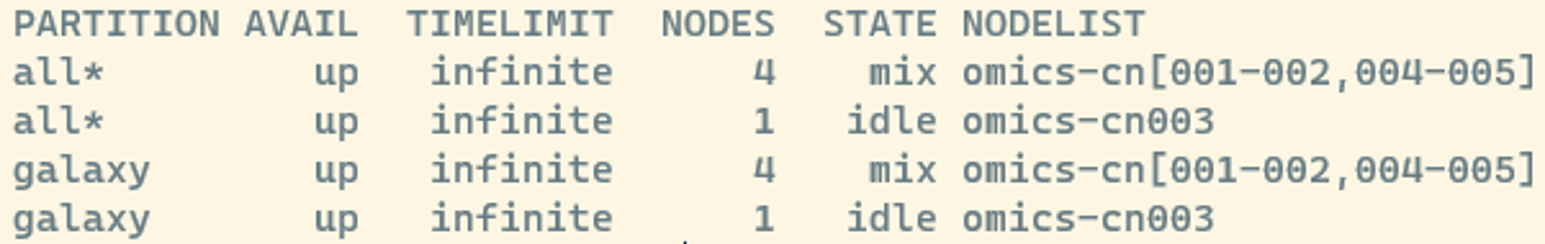
\includegraphics[width=0.7\textwidth,height=\textheight]{../img/sinfo.png}
\end{center}

Here, you see information about the:

\begin{itemize}
\tightlist
\item
  partition: the queues that are available
\item
  state: if a node is busy or not

  \begin{itemize}
  \tightlist
  \item
    mix : consumable resources partially allocated
  \item
    idle : available to requests consumable resources
  \item
    drain : unavailable for use per system administrator request
  \item
    alloc : consumable resources fully allocated
  \item
    down : unavailable for use.
  \end{itemize}
\item
  Nodes: The number of nodes
\item
  NodeList: the names of the nodes omics-cn001 to omics-cn005
\end{itemize}

\subsection{View info about jobs in the
queue}\label{view-info-about-jobs-in-the-queue}

The following command gives us some information about how busy the HPC
is:

\begin{Shaded}
\begin{Highlighting}[]
\ExtensionTok{squeue}
\end{Highlighting}
\end{Shaded}

After running this, you can see all jobs scheduled on the HPC:

\begin{center}
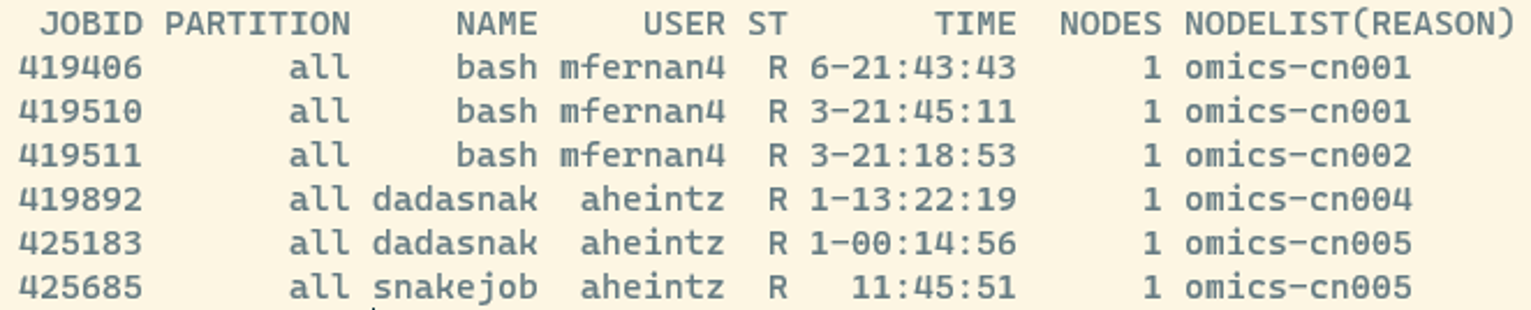
\includegraphics[width=0.9\textwidth,height=\textheight]{../img/squeue.png}
\end{center}

\begin{itemize}
\tightlist
\item
  JOBID: every job gets a number and you can manipulate jobs via this
  number
\item
  ST: Job state codes that describe the current state of the job. The
  full list of abbreviations can be found
  \href{https://curc.readthedocs.io/en/latest/running-jobs/squeue-status-codes.html}{here}
\end{itemize}

If we would have submitted a job, we also should see it running.

\section{\texorpdfstring{\texttt{srun}: submitting a job
interactively}{srun: submitting a job interactively}}\label{srun-submitting-a-job-interactively}

\texttt{srun} is used when you want to run tasks interactively or have
more control over the execution. You directly issue srun commands in the
terminal, specifying the tasks to be executed and their resource
requirements.

Use \texttt{srun} when:

\begin{itemize}
\tightlist
\item
  You want to run tasks interactively and need immediate feedback.
\item
  You are testing or debugging your commands before incorporating them
  into a script.
\item
  You need more control over the execution of tasks.
\end{itemize}

Let's submit a very simple example for which we would not even need to
submit a job, but just to get you started.

\begin{Shaded}
\begin{Highlighting}[]
\ExtensionTok{srun}\NormalTok{ echo }\StringTok{"Hello interactively"}
\end{Highlighting}
\end{Shaded}

You should see the output of echo printed to the screen and if you would
run \texttt{squeue} you won't even see your job since everything ran so
fast. Now assume you want to run a more complex interactive task with
srun then it is good to specify the resources your job needs by adding
flags, i.e.

\begin{Shaded}
\begin{Highlighting}[]
\ExtensionTok{srun} \AttributeTok{{-}{-}nodes}\OperatorTok{=}\NormalTok{1 }\AttributeTok{{-}{-}ntasks}\OperatorTok{=}\NormalTok{1 }\AttributeTok{{-}{-}cpus{-}per{-}task}\OperatorTok{=}\NormalTok{1 }\AttributeTok{{-}{-}mem}\OperatorTok{=}\NormalTok{1G echo }\StringTok{"Hello interactively"}
\end{Highlighting}
\end{Shaded}

Here, each flag means the following:

\begin{itemize}
\tightlist
\item
  \texttt{-\/-nodes=1}: Specifies the number of nodes. In this case,
  it's set to 1 and tells slurm that we want to use a full node. Only
  use this if you make use of all resources on that node, otherwise
  omit.
\item
  \texttt{-\/-ntasks=1}: Defines the number of tasks to run. Here, it's
  set to 1 since we want to use echo once
\item
  \texttt{-\/-cpus-per-task=1}: Specifies the number of CPUs per task.
  Adjust this based on the computational requirements of your task
\item
  \texttt{-\/-mem=1G}: Sets the memory requirement for the task. Modify
  this based on your task's memory needs
\item
  \texttt{echo\ "Hello\ interactively}: The actual command you want to
  run interactively
\end{itemize}

\subsection{Choosing the right amount of
resources}\label{choosing-the-right-amount-of-resources}

When you're just starting, deciding on the right resources to request
for your computational job can be a bit challenging. The resource
requirements can vary significantly based on the specific tool or
workflow you are using. Here are some general guidelines to help you
make informed choices:

\begin{itemize}
\tightlist
\item
  Use default settings: Begin by working with the default settings
  provided by the HPC cluster. These are often set to provide a balanced
  resource allocation for a wide range of tasks
\item
  Check the software documentation: Consult the documentation of the
  software or tool you are using. Many tools provide recommendations for
  resource allocation based on the nature of the computation.
\item
  Testing with Small Datasets: For initial testing and debugging,
  consider working with a smaller subset of your dataset. This allows
  for faster job turnaround times, helping you identify and resolve
  issues more efficiently.
\item
  Monitor the resources usage:

  \begin{itemize}
  \tightlist
  \item
    Use \texttt{sacct} to check what resources a finished job has used.
    Look for columns like MaxRSS (maximum resident set size) to check if
    the amount of memory allocated (--mem) was appropriate. An example
    command would be
    \texttt{sacct\ -j\ 419847\ -\/-format=User,JobID,Jobname,state,start,end,elapsed,MaxRss,nnodes,ncpus,nodelist}
  \item
    For instance, if you would have used
    \texttt{-\/-cpus-per-task=4\ -\/-mem=4G}, you would expect to use a
    total of 16 GB of memory (4 CPUs * 4 GB). Verify this with sacct to
    ensure your job's resource requirements align with its actual usage.
  \end{itemize}
\item
  Fine-Tuning Resource Requests: If you encounter performance issues or
  your jobs are not completing successfully, consider iteratively
  adjusting resource requests. This might involve increasing or
  decreasing the number of CPUs, memory allocation, or other relevant
  parameters.
\end{itemize}

\subsection{Run FastQC with srun}\label{run-fastqc-with-srun}

\href{https://www.bioinformatics.babraham.ac.uk/projects/fastqc/}{FastQC}
is a quality control tool for high throughput sequence data that is
already installed on crunchomics. Let's use this to run an actually
software on our data.

\begin{Shaded}
\begin{Highlighting}[]
\FunctionTok{mkdir} \AttributeTok{{-}p}\NormalTok{ results/fastqc }

\ExtensionTok{srun} \AttributeTok{{-}{-}cpus{-}per{-}task}\OperatorTok{=}\NormalTok{1 }\AttributeTok{{-}{-}mem}\OperatorTok{=}\NormalTok{5G fastqc data/seq\_project/}\PreprocessorTok{*}\NormalTok{/}\PreprocessorTok{*}\NormalTok{gz }\AttributeTok{{-}o}\NormalTok{ results/fastqc  }\AttributeTok{{-}{-}threads}\NormalTok{ 1}

\ExtensionTok{ll}\NormalTok{ results/fastqc /}\PreprocessorTok{*}
\end{Highlighting}
\end{Shaded}

Since we work with little data this will run extremely fast, however, if
you would be logged into Crunchomics via a second window and run
\texttt{squeue} you should see that your job is actively running:

\begin{center}
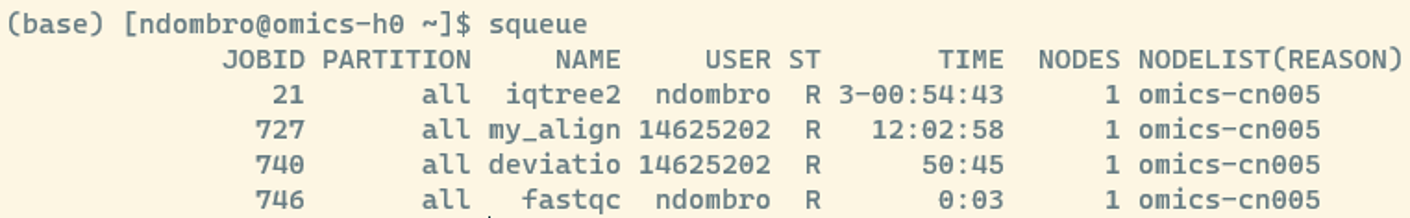
\includegraphics[width=0.7\textwidth,height=\textheight]{../img/squeue2.png}
\end{center}

Additionally, after the run is completed, you should see that several
html files were generated in our fastqc folder.

\begin{tcolorbox}[enhanced jigsaw, coltitle=black, leftrule=.75mm, colback=white, toptitle=1mm, breakable, toprule=.15mm, colbacktitle=quarto-callout-caution-color!10!white, bottomtitle=1mm, arc=.35mm, opacitybacktitle=0.6, bottomrule=.15mm, titlerule=0mm, title=\textcolor{quarto-callout-caution-color}{\faFire}\hspace{0.5em}{Exercise}, rightrule=.15mm, left=2mm, colframe=quarto-callout-caution-color-frame, opacityback=0]

Use scp to download the data to your own computer and view one of the
html files.

Click me to see an answer

\begin{Shaded}
\begin{Highlighting}[]
\FunctionTok{scp}\NormalTok{ username@omics{-}h0.science.uva.nl:/home/username/personal/projectX/results/fastqc/}\PreprocessorTok{*}\NormalTok{html results/fastqc/}
\end{Highlighting}
\end{Shaded}

You could also open a file on Crunchomics with
\texttt{firefox\ results/fastqc/Sample-DUMMY1\_R1\_fastqc.html}.
However, connecting to the internet via a cli on a remote server tends
to be rather slow and its often better to view files to your own
computer especially if they are large files.

If you want to know more about how to to interprete the output, you can
visit
\href{https://www.bioinformatics.babraham.ac.uk/projects/fastqc/}{the
fastqc website}, which gives some examples for interpreting good and bad
reports.

\end{tcolorbox}

\section{\texorpdfstring{\texttt{screen}: Submitting long running jobs
via
srun}{screen: Submitting long running jobs via srun}}\label{screen-submitting-long-running-jobs-via-srun}

One down-side of \texttt{srun} for long running jobs is that your
terminal gets ``blocked'' as long as the job is running and that your
job is lost if you loose the ssh connection to the HPC. For long running
jobs, there are two ways to deal with this:

\begin{enumerate}
\def\labelenumi{\arabic{enumi}.}
\tightlist
\item
  submit a srun job in a screen
\item
  use sbatch
\end{enumerate}

In this section, we will cover how to use Screen. Screen or GNU Screen
is a terminal multiplexer. This means that you can start a screen
session and then open any number of windows (virtual terminals) inside
that session.

Processes running in Screen will continue to run when their window is
not visible even if you get disconnected. This is perfect, if we start
longer running processes on the server and want to shut down our
computer when leaving for the day. As long as the server is still
connected to the internet, your process will continue running.

We start a screen as follows:

\begin{Shaded}
\begin{Highlighting}[]
\ExtensionTok{screen}
\end{Highlighting}
\end{Shaded}

We detach (go outside of a screen but keep the screen running in the
background) from a screen with \texttt{control+a+d}.

If you run multiple things, it can be useful to give your screens more
descriptive names. You can do this as follows:

\begin{Shaded}
\begin{Highlighting}[]
\CommentTok{\#start a screen and give it a name}
\ExtensionTok{screen} \AttributeTok{{-}S}\NormalTok{ run\_fastqc}
\end{Highlighting}
\end{Shaded}

After detaching from a screen you can list all currently running screens
with:

\begin{Shaded}
\begin{Highlighting}[]
\ExtensionTok{screen} \AttributeTok{{-}ls}
\end{Highlighting}
\end{Shaded}

You can restart a screen like this:

\begin{Shaded}
\begin{Highlighting}[]
\CommentTok{\#restart an existing screen}
\ExtensionTok{screen} \AttributeTok{{-}r}\NormalTok{ run\_fastqc}
\end{Highlighting}
\end{Shaded}

Now inside our screen, we can run fastqc same as we did before:

\begin{Shaded}
\begin{Highlighting}[]
\ExtensionTok{srun} \AttributeTok{{-}{-}cpus{-}per{-}task}\OperatorTok{=}\NormalTok{1 }\AttributeTok{{-}{-}mem}\OperatorTok{=}\NormalTok{5G fastqc data/seq\_project/}\PreprocessorTok{*}\NormalTok{/}\PreprocessorTok{*}\NormalTok{gz }\AttributeTok{{-}o}\NormalTok{ results/fastqc  }\AttributeTok{{-}{-}threads}\NormalTok{ 1 }
\end{Highlighting}
\end{Shaded}

And for long-running jobs we can jump inside and outside of the job,
while it is running and at the same time do other things from the cli.

If you want to completely close and remove a screen, type the following
while being inside of the screen:

\begin{Shaded}
\begin{Highlighting}[]
\BuiltInTok{exit}
\end{Highlighting}
\end{Shaded}

\section{\texorpdfstring{\texttt{sbatch}: submitting a
job}{sbatch: submitting a job}}\label{sbatch-submitting-a-job}

\texttt{sbatch} is your go-to command when you have a script (a batch
script) that needs to be executed without direct user interaction.

Use sbatch when:

\begin{itemize}
\tightlist
\item
  You have long-running or resource-intensive tasks.
\item
  You want to submit jobs that can run independently without your
  immediate supervision
\item
  You want to submit multiple jobs at once
\end{itemize}

To run a job script, you:

\begin{itemize}
\tightlist
\item
  create a script that contains all the commands and configurations
  needed for your job
\item
  use sbatch to submit this script to the Slurm scheduler, and it takes
  care of the rest.
\end{itemize}

Let's start with having some good folder organization to keep our
project folder organized:

\begin{Shaded}
\begin{Highlighting}[]
\FunctionTok{mkdir}\NormalTok{ scripts }
\FunctionTok{mkdir}\NormalTok{ logs}
\end{Highlighting}
\end{Shaded}

To get started, assume we have created a script named
\texttt{run\_fastqc.sh} with the following content in which we want to
run fastqc. Notice, how in this script I added some additional commands.
Here, I just use this to print some information about the progress which
could be printed to a log file but if you have several commands that
should be executed after each other that is how you could do it.

\begin{Shaded}
\begin{Highlighting}[]
\CommentTok{\#!/bin/bash}
\CommentTok{\#SBATCH {-}{-}cpus{-}per{-}task=2}
\CommentTok{\#SBATCH {-}{-}mem=5G}

\BuiltInTok{echo} \StringTok{"Start fastqc"}

\ExtensionTok{srun} \AttributeTok{{-}{-}cpus{-}per{-}task}\OperatorTok{=}\NormalTok{1 }\AttributeTok{{-}{-}mem}\OperatorTok{=}\NormalTok{5G fastqc data/seq\_project/}\PreprocessorTok{*}\NormalTok{/}\PreprocessorTok{*}\NormalTok{gz }\AttributeTok{{-}o}\NormalTok{ results/fastqc  }\AttributeTok{{-}{-}threads}\NormalTok{ 1}

\BuiltInTok{echo} \StringTok{"fastqc finished"}
\end{Highlighting}
\end{Shaded}

To prepare the script:

\begin{itemize}
\tightlist
\item
  run \texttt{nano\ scripts/run\_fastqc.sh}.
\item
  Copy and paste the content you see above.
\item
  Press \texttt{ctrl+x} to exit nano
\item
  Type \texttt{Y} when prompted if the changes should be saved.
\item
  Confirm the name by pressing enter
\end{itemize}

The we can submit \texttt{run\_fastqc.sh} with:

\begin{Shaded}
\begin{Highlighting}[]
\CommentTok{\#submit job: 754}
\ExtensionTok{sbatch}\NormalTok{ sbatch scripts/run\_fastqc.sh}

\CommentTok{\#check if job is running correctly}
\ExtensionTok{squeue}
\end{Highlighting}
\end{Shaded}

After running this, you should see that the job was submitted and
something like this printed to the screen
\texttt{Submitted\ batch\ job\ 754}.

You will also see that a new file is generated that will look something
like this \texttt{slurm-425707.out}. When you submit a batch job using
sbatch, Slurm redirects the standard output and standard error streams
of your job to a file named in the format slurm-JOBID.out, where JOBID
is the unique identifier assigned to your job.

This file is useful as it:

\begin{itemize}
\tightlist
\item
  Captures the output of our batch scripts and stores them in a file
\item
  Can be used for debugging, since if something goes wrong with your
  job, examining the contents of this file can provide valuable insights
  into the issue. Error messages, warnings, or unexpected outputs are
  often recorded here.
\end{itemize}

Feel free to explore the content of the log file, do you see how the
echo commands are used as well?

\begin{tcolorbox}[enhanced jigsaw, coltitle=black, leftrule=.75mm, colback=white, toptitle=1mm, breakable, toprule=.15mm, colbacktitle=quarto-callout-tip-color!10!white, bottomtitle=1mm, arc=.35mm, opacitybacktitle=0.6, bottomrule=.15mm, titlerule=0mm, title=\textcolor{quarto-callout-tip-color}{\faLightbulb}\hspace{0.5em}{Tip: sbatch and better log files}, rightrule=.15mm, left=2mm, colframe=quarto-callout-tip-color-frame, opacityback=0]

We have seen that by default sbatch redirects the standard output and
error to our working directory and that it decides itself how to name
the files. Since file organization is very important, you find below an
example to:

\begin{itemize}
\tightlist
\item
  Store the standard output and error in two separate files
\item
  Redirect the output into another folder, the logs folder
\item
  In the code below, the \texttt{\%j} is replaced with the job
  allocation number
\end{itemize}

\begin{Shaded}
\begin{Highlighting}[]
\CommentTok{\#!/bin/bash}
\CommentTok{\#SBATCH {-}{-}job{-}name=our\_fastqc\_job}
\CommentTok{\#SBATCH {-}{-}output=logs/fastqc\_\%j.out}
\CommentTok{\#SBATCH {-}{-}error=logs/fastqc\_\%j.err}
\CommentTok{\#SBATCH {-}{-}cpus{-}per{-}task=2}
\CommentTok{\#SBATCH {-}{-}mem=5G}

\BuiltInTok{echo} \StringTok{"Start fastqc"}

\ExtensionTok{srun} \AttributeTok{{-}{-}cpus{-}per{-}task}\OperatorTok{=}\NormalTok{1 }\AttributeTok{{-}{-}mem}\OperatorTok{=}\NormalTok{5G fastqc data/seq\_project/}\PreprocessorTok{*}\NormalTok{/}\PreprocessorTok{*}\NormalTok{gz }\AttributeTok{{-}o}\NormalTok{ results/fastqc  }\AttributeTok{{-}{-}threads}\NormalTok{ 1}

\BuiltInTok{echo} \StringTok{"fastqc finished"}
\end{Highlighting}
\end{Shaded}

\end{tcolorbox}

\begin{tcolorbox}[enhanced jigsaw, coltitle=black, leftrule=.75mm, colback=white, toptitle=1mm, breakable, toprule=.15mm, colbacktitle=quarto-callout-tip-color!10!white, bottomtitle=1mm, arc=.35mm, opacitybacktitle=0.6, bottomrule=.15mm, titlerule=0mm, title=\textcolor{quarto-callout-tip-color}{\faLightbulb}\hspace{0.5em}{Advanced tip: sbatch and multiple files}, rightrule=.15mm, left=2mm, colframe=quarto-callout-tip-color-frame, opacityback=0]

With fastqc we are very lucky that it can identify all the fastq files
in the directory we specify with \texttt{-o} and use a wildcard. This is
extremely useful for us but by far not all programs work this way.

For this section, lets assume that we need to provide each individual
file we want to analyse, one by one. How would we run such a job
effectively?

What we want to do is created what is called a job array that allows us
to:

\begin{itemize}
\tightlist
\item
  Run multiple jobs that have the same job definition, i.e.~cpus, memory
  and software used
\item
  Run these job in the most optimal way. I.e. we do not want to run one
  job after each other but we also want to run jobs in parallel at the
  same time to optimize resource usage.
\end{itemize}

Let's start with making a list with files we want to work with based on
what we have already learned:

\begin{Shaded}
\begin{Highlighting}[]
\FunctionTok{ls}\NormalTok{ data/seq\_project/}\PreprocessorTok{*}\NormalTok{/}\PreprocessorTok{*}\NormalTok{.gz }\KeywordTok{|} \FunctionTok{cut} \AttributeTok{{-}f4} \AttributeTok{{-}d} \StringTok{"/"} \OperatorTok{\textgreater{}}\NormalTok{ samples.txt}
\end{Highlighting}
\end{Shaded}

Next, we can use this text file in our job array, the content of which
we store in \texttt{scripts/array.sh}:

\begin{Shaded}
\begin{Highlighting}[]
\CommentTok{\#!/bin/bash}

\CommentTok{\#SBATCH {-}{-}job{-}name=my\_array}
\CommentTok{\#SBATCH {-}{-}output=logs/array\_\%A\_\%a.out}
\CommentTok{\#SBATCH {-}{-}error=logs/array\_\%A\_\%a.err}
\CommentTok{\#SBATCH {-}{-}array=1{-}8}
\CommentTok{\#SBATCH {-}{-}cpus{-}per{-}task=1}
\CommentTok{\#SBATCH {-}{-}mem{-}per{-}cpu=5G}

\CommentTok{\#calculate the index of the current job within the batch}
\CommentTok{\#in our case the index will store the values 1 to 8}
\VariableTok{INDEX}\OperatorTok{=}\VariableTok{$((SLURM\_ARRAY\_TASK\_ID} \VariableTok{))}

\CommentTok{\#build array structure via ale file names}
\VariableTok{CURRENT\_SAMPLE}\OperatorTok{=}\VariableTok{$(}\FunctionTok{cat}\NormalTok{ samples.txt }\KeywordTok{|}  \FunctionTok{sed} \AttributeTok{{-}n} \StringTok{"}\VariableTok{$\{INDEX\}}\StringTok{p"}\VariableTok{)}

\CommentTok{\#print what is actually happening}
\BuiltInTok{echo} \StringTok{"Now Job}\VariableTok{$\{INDEX\}}\StringTok{ runs on }\VariableTok{$\{CURRENT\_SAMPLE\}}\StringTok{"}

\CommentTok{\#run the actual job}
\ExtensionTok{fastqc}\NormalTok{ data/seq\_project/}\PreprocessorTok{*}\NormalTok{/}\VariableTok{$\{CURRENT\_SAMPLE\}} \AttributeTok{{-}o}\NormalTok{ results/fastqc  }\AttributeTok{{-}{-}threads}\NormalTok{ 1}
\end{Highlighting}
\end{Shaded}

In the script we use some new SLURM arguments:

\begin{itemize}
\tightlist
\item
  \texttt{\#SBATCH\ -\/-array=1-8}: Sets up a job array, specifying the
  range (1-8). We choose 1-8 because we have exactly 8 fastq.gz files we
  want to analyse
\item
  \texttt{\#SBATCH\ -\/-output=logs/array\_\%A\_\%a.out}: Store the
  standard output and error. \texttt{\%A} represents the job ID assigned
  by Slurm, and \texttt{\%a} represents the array task ID
\end{itemize}

The job does the following:

\begin{itemize}
\tightlist
\item
  The \texttt{INDEX} variable is storing the value of the current
  \texttt{SLURM\_ARRAY\_TASK\_ID}. This represents the ID of the current
  job within the array. In our case this will be first 1, then 2,
  \ldots, and finally 3.
\item
  Next, we build the array structure:

  \begin{itemize}
  \tightlist
  \item
    The \texttt{CURRENT\_SAMPLE} variable is created by reading the
    \texttt{sample\_list.txt} file with \texttt{cat}.
  \item
    We then use a pipe to extract the sample at the calculated index
    using sed.
    \href{https://scienceparkstudygroup.github.io/software_information/source/cli/cli_file_manipulation.html\#sed-manipulating-the-content-of-files}{Sed}
    is an extremly powerful way to edit text that we have not yet
    covered but \texttt{-n\ 1p} is a option that allows us to print one
    specific line of a file, here the first one when running array 1. So
    for the first array the actual code run is the following
    \texttt{cat\ samples.txt\ \textbar{}\ \ sed\ -n\ "1p"}. For the next
    array, we would run
    \texttt{cat\ samples.txt\ \textbar{}\ \ sed\ -n\ "2p"} and so forth.
  \item
    The output of the pipe is stored in a variable, called
    \texttt{CURRENT\_SAMPLE}. For our first sample this will be
    \texttt{Sample-DUMMY1\_R1.fastq.gz}
  \end{itemize}
\item
  We use echo to record what was executed when to store it in the
  standard output
\item
  We run our actual fastqc job on the file name that is currently stored
  in the \texttt{CURRENT\_SAMPLE} variable.
\end{itemize}

If we check what is happening right after submitting the job with
\texttt{squeue} we should see something like this:

\begin{center}
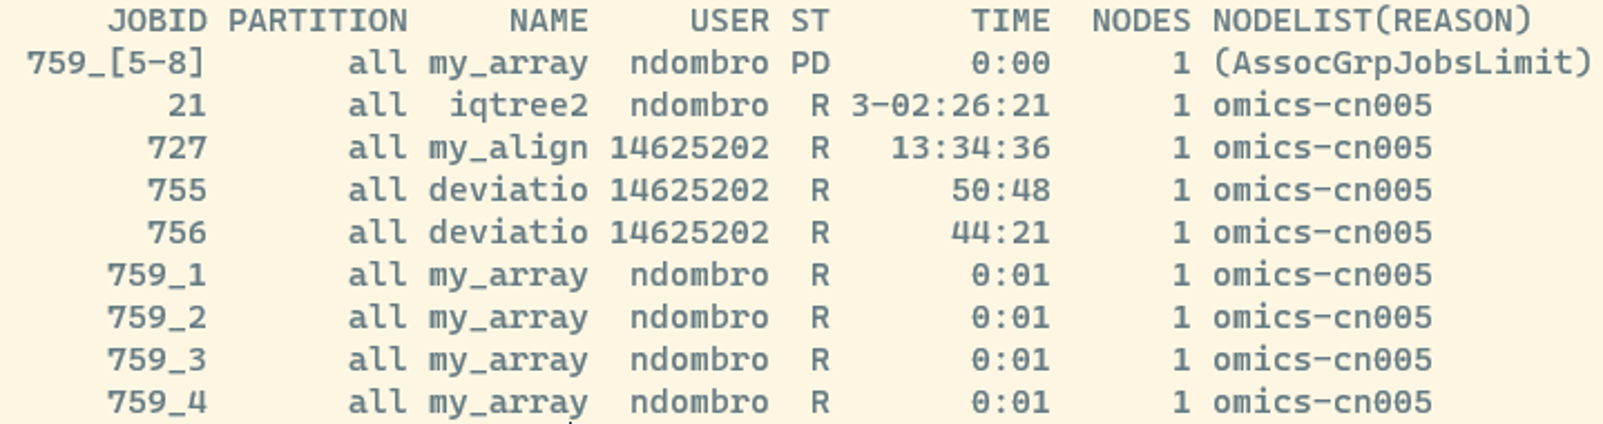
\includegraphics[width=0.7\textwidth,height=\textheight]{../img/arrays.png}
\end{center}

We see that jobs 1-4 are already running and the other jobs are
currently waiting for space.

If we check the log files we should see:

\begin{center}
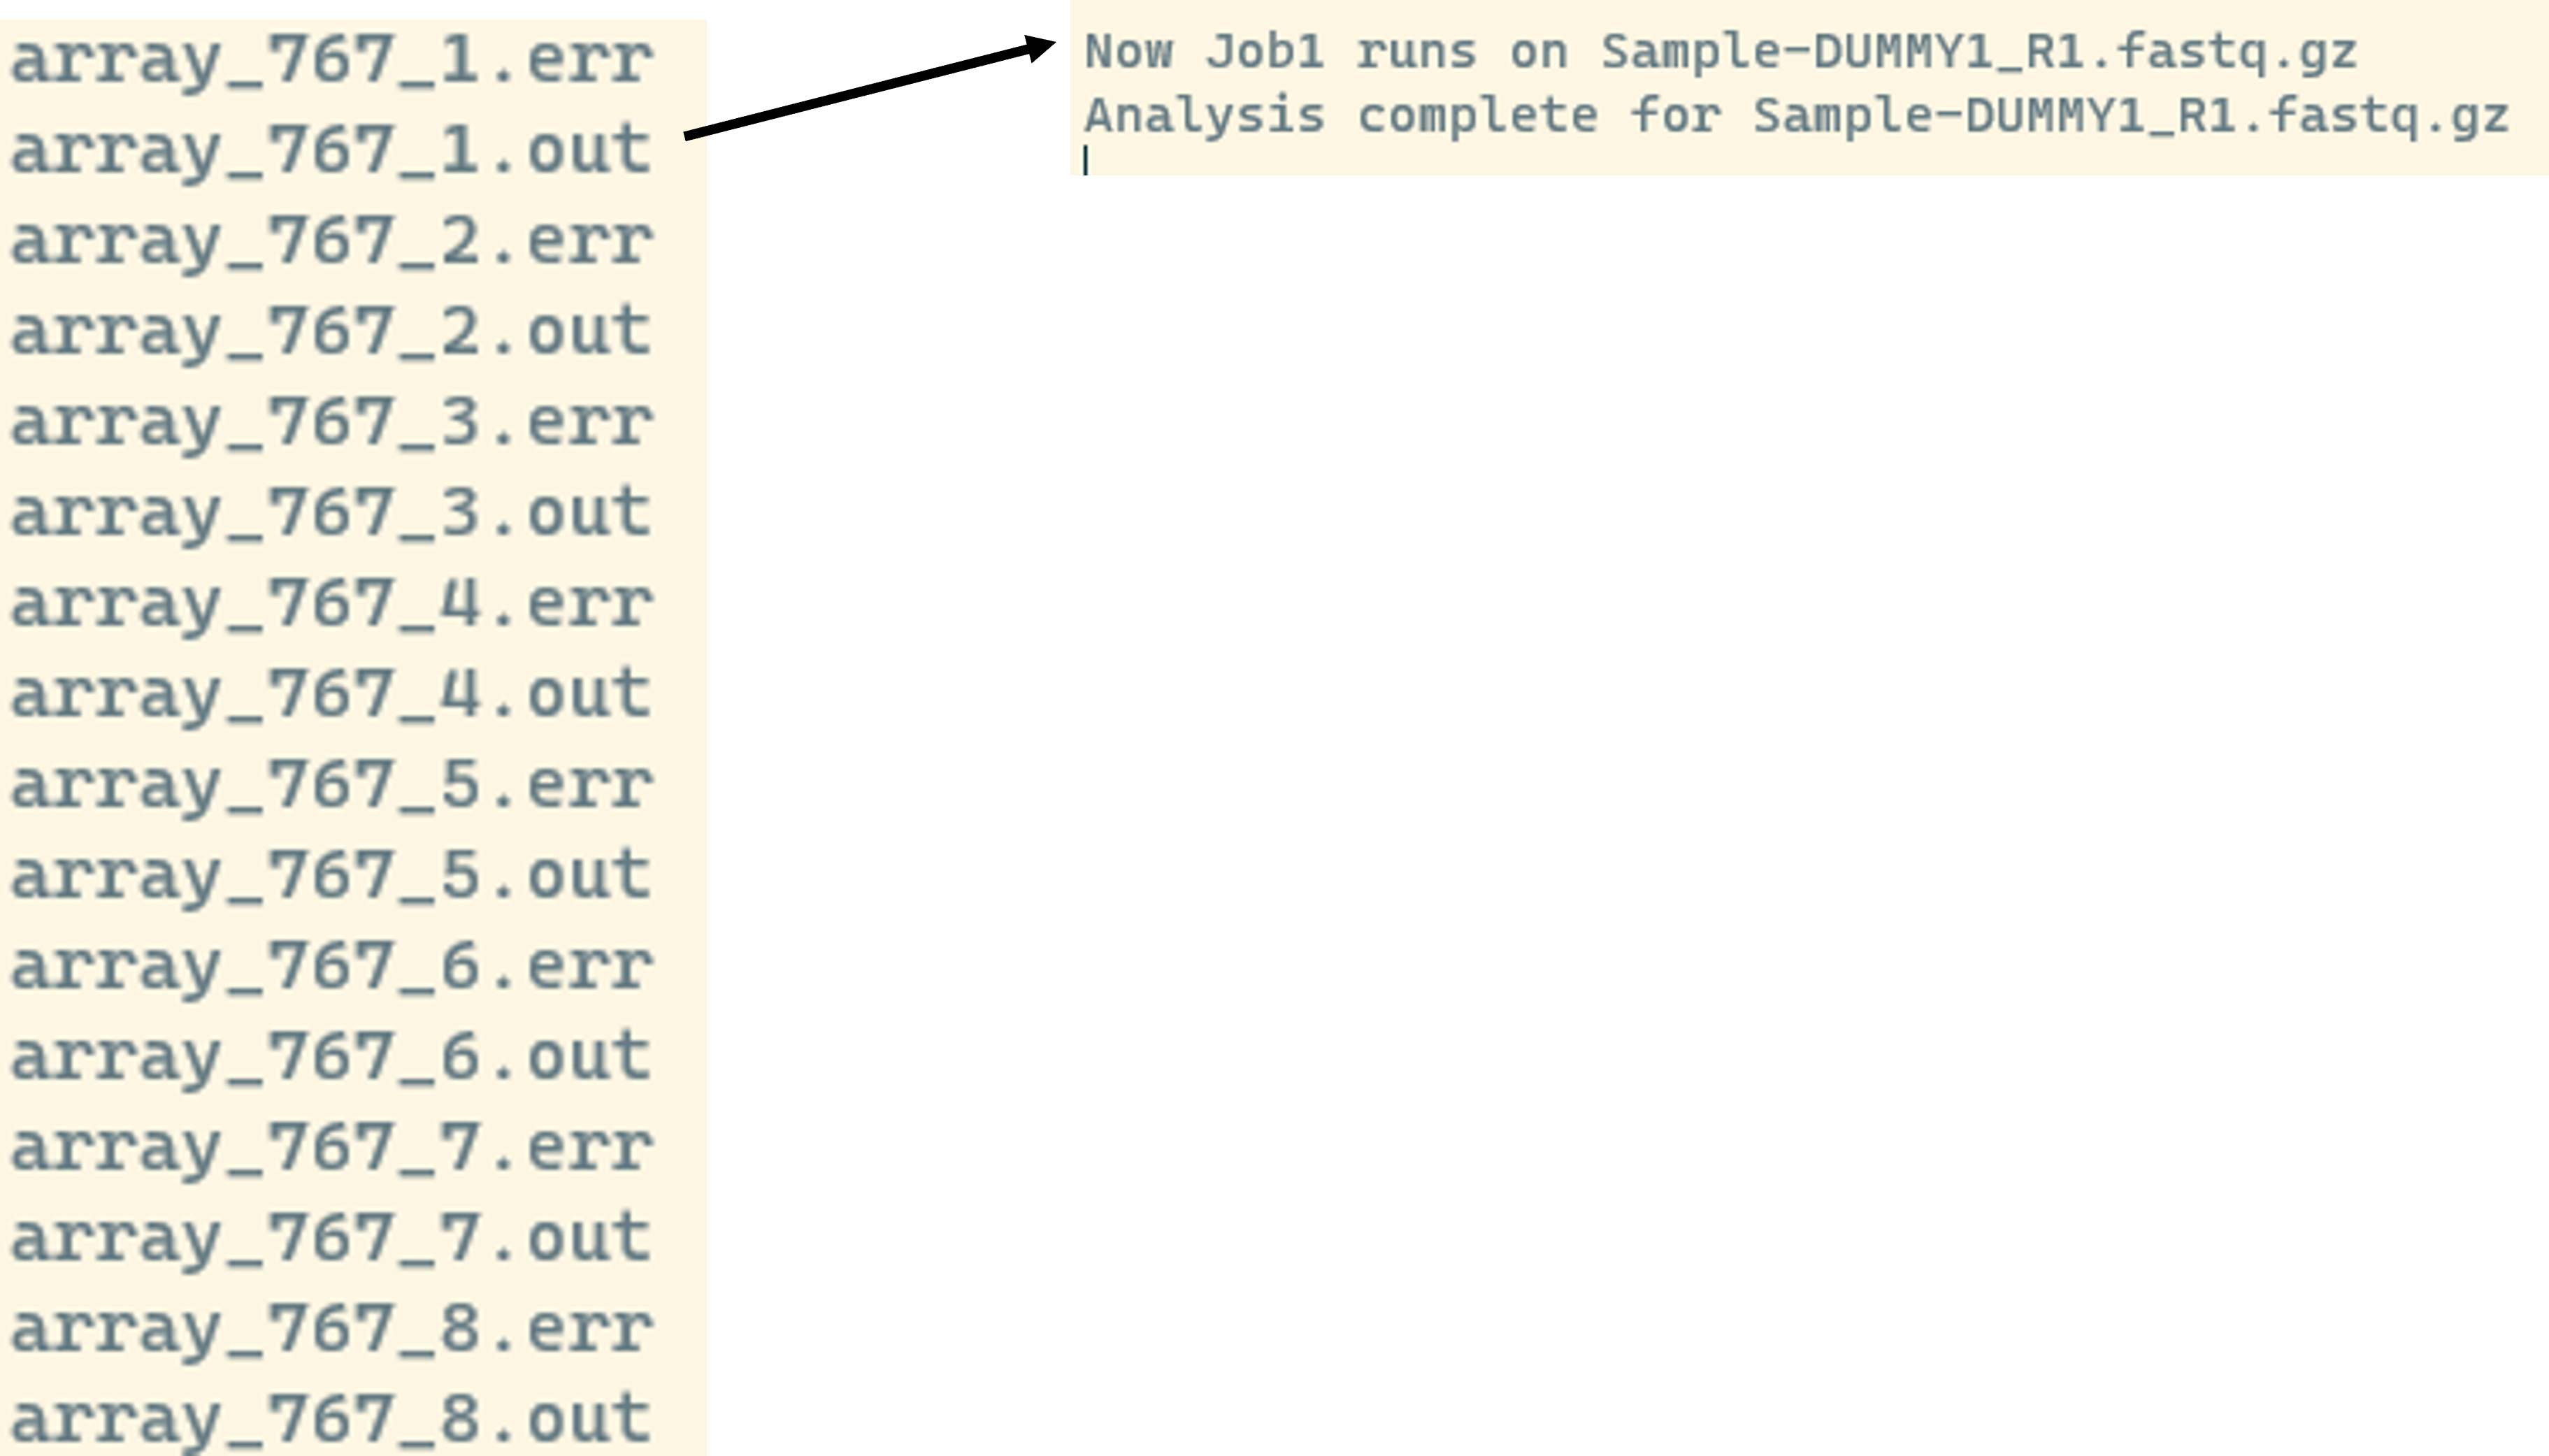
\includegraphics[width=0.7\textwidth,height=\textheight]{../img/arrays2.png}
\end{center}

We see that we get an individual output and error file for each job. In
the output we see what value is stored in the \texttt{INDEX}, here 1,
and the \texttt{CURRENT\_SAMPLE}, here
\texttt{Sample-DUMMY1\_R1.fastq.gz}.

\end{tcolorbox}



\end{document}
